\section{Logging}
\subsection{fluentd}
\subsubsection{Decision Log}
First we tried to implement our logging with kibana and elastic search, which worked on our local machines. The problem with this was that we only had 1GB RAM on our web server, 
which wasn't enough to run elastic search. To resolve that issue we looked for other technologies like fluentd. \

When facing implementing logging to a system several challenges come up, for example there are disparate log formats of different applications, 
logs that are scattered across multiple sources (data fragmentation), reliability concerns like network outages and routing different logs to different destinations 
based on the application or service. \

In order to manage these difficulties we decided to use fluentd. Fluentd is an open source data collector which processes the data from various sources, 
making it easier to manage and analyze. The following aspects show why fluentd is so powerful: 

\begin{itemize}
    \item \textbf{Unified Logging Layer:} Fluentd provides a unified platform for collecting, transforming, and routing logs from diverse sources, simplifying the log management process.
    
    \item \textbf{Data Agnosticism:} Regardless of the data source—be it Prometheus metrics, Grafana dashboards, or application logs—Fluentd seamlessly collects and processes data in a unified format, fostering interoperability and ease of analysis.
    
    \item \textbf{Configurable Routing:} With Fluentd, we could effortlessly configure log routing based on application or service, directing logs to specific destinations for centralized storage and analysis.
    
    \item \textbf{Flexibility:} Fluentd's versatility enables us to send data from any source to any destination, empowering us to adapt to evolving logging requirements seamlessly.
\end{itemize}

\subsubsection{Implementation of fluentd}
\begin{center}
    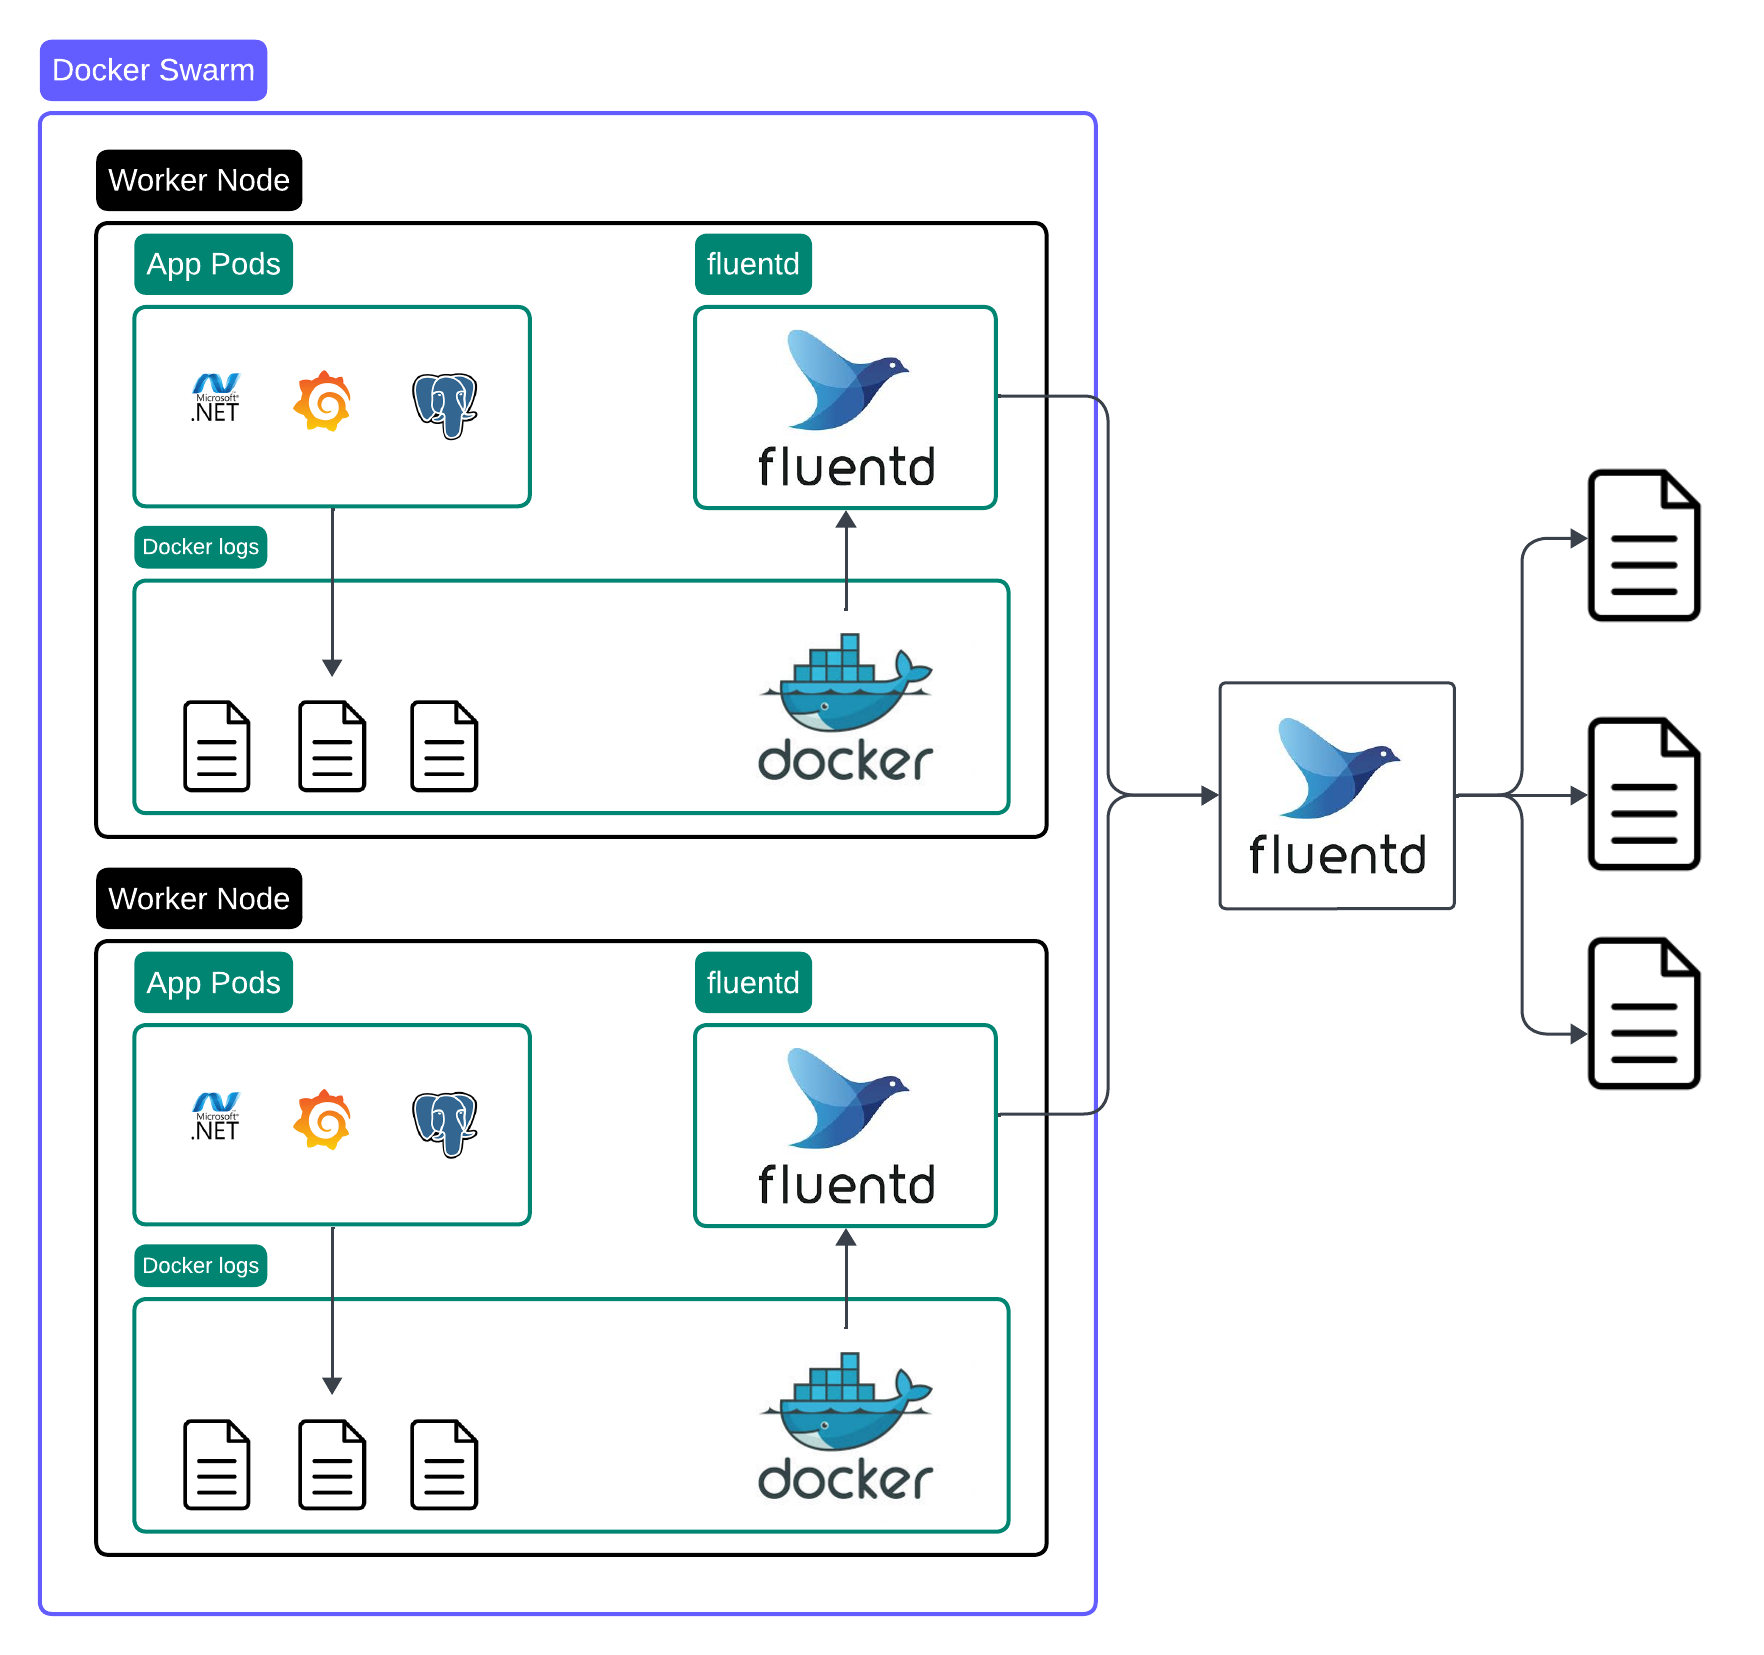
\includegraphics[width=1\textwidth]{Logging2.png}
\end{center}
\subsubsection*{Fluentd Configuration}
Fluentd is configured to listen for incoming log data via the forward input plugin on port 24224. Log data from different sources 
(minitwit-database, minitwit-service, prometheus, grafana) is matched using the match directive which specifies the destination path and format for the corresponding log data. 
Log data is buffered using the buffer directive to handle data spikes or network outages, ensuring reliable log collection.

\subsubsection*{Docker Compose Configuration}
A fluentd container is defined using the fluent/fluentd:v1.12-debian image. Each service in the Docker Compose file depends on the fluentd service for logging. 
Logging is configured to use fluentd as the logging driver, with specific options (fluentd-async-connect, fluentd-retry-wait, fluentd-max-retries) to ensure reliable log transmission. 
Each service specifies a unique tag to route log data to the appropriate destination, which in our case are simple log files, in fluentd based on the matching 
rules defined in the fluentd.conf file.